\section{Method}
\label{sec:method}

Fig.~\ref{fig:pipeline} shows the three stages. Reasoning produces a structured description of the clip and a list of candidate variations. Guidance converts that description into a prompt and a set of control maps. Generation renders the variant. Every input to the generator is produced by an earlier stage; the only manual decision is which variation to render.

\begin{figure}[t]
\centering
\begin{tikzpicture}[
  node distance=5mm and 4mm,
  box/.style={draw, rounded corners=2pt, align=center, font=\footnotesize, inner sep=2pt, minimum height=12mm, text width=21mm},
  model/.style={box, fill=black!8},
  data/.style={box, fill=white},
  arr/.style={-{Latex[length=1.8mm]}, thick}
]
% row 1: reasoning
\node[data] (clip) {Egocentric clip $V$\\60 frames, 4 fps};
\node[model, right=of clip] (reason) {Cosmos 3 Nano\\reasoning tower};
\node[data, right=of reason] (onto) {Ontology $\mathcal{O}$\\objects, boxes,\\variations};
\node[model, right=of onto] (llm) {GPT-4o mini\\filter + prompt};
% row 2: mask and prompt
\node[model, below=of reason] (sam) {SAM2\\box $\to$ tracked mask};
\node[data, right=of sam] (mask) {Mask $M$\\(subtraction)};
\node[data, right=of mask] (prompt) {Prompt $p$};
% row 3: controls and generation
\node[model, below=of sam] (pre) {Canny / depth / blur};
\node[data, right=of pre] (ctrl) {Controls\\$c_{\mathrm{edge}}, c_{\mathrm{depth}},$\\$c_{\mathrm{vis}}$};
\node[model, right=of ctrl] (transfer) {Cosmos\\Transfer 2.5\\weights $w$};
\node[data, right=of transfer, text width=14mm] (out) {Variant $V'$};
\draw[arr] (clip) -- (reason);
\draw[arr] (reason) -- (onto);
\draw[arr] (onto) -- (llm);
\draw[arr] (llm) -- (prompt);
\draw[arr] (onto.south) -- ++(0,-2.5mm) -| (sam.north);
\draw[arr] (sam) -- (mask);
\draw[arr] (clip.south) |- (pre.west);
\draw[arr] (pre) -- (ctrl);
\draw[arr] (ctrl) -- (transfer);
\draw[arr] (prompt.south) -- ([xshift=5mm]transfer.north);
\draw[arr] (mask.south) -- ++(0,-2.5mm) -| ([xshift=-6mm]transfer.north);
\draw[arr] (transfer) -- (out);
\end{tikzpicture}
\caption{Pipeline. The ontology produced by the reasoning stage drives both the text prompt and the segmentation mask, so the same structured output decides what changes and what is held fixed. The mask $M$ enters the renderer as its segmentation control; the weights $w$ are given in Table~\ref{tab:weights}.}
\label{fig:pipeline}
\end{figure}

\subsection{Notation}
A clip is a frame sequence $V=\{I_t\}_{t=1}^{T}$ with $T=60$ at 4~fps and resolution $854\times480$. The reasoning model $R$ maps the first frame to an ontology $\mathcal{O}=R(I_1)$ containing a task record, a set of objects $\{o_k\}$ with normalized boxes $b_k\in[0,1000]^4$, and for each object a set of candidate variations $\mathcal{U}_k$. A variation $u\in\mathcal{U}_k$ is a short phrase such as ``solid blue matte.'' The prompt writer $L$ maps $(\mathcal{O},u)$ to a text prompt $p$. The segmenter $S$ maps a box and the clip to a tracked binary mask $S(b_k,V)\in\{0,1\}^{T\times H\times W}$. The generator $G$ maps $(V,p,\{c_j\},w)$ to a variant $V'$, where $c_j$ are control videos and $w$ their weights.

\subsection{Reasoning: from clip to ontology}
\label{sec:reason}
We prompt the reasoning tower of Cosmos 3 Nano~\cite{cosmos3,cosmos3nano} (16B parameters total, 8B in the reasoning tower) with the first frame of the clip and a fixed instruction (Appendix~\ref{app:prompt}). The instruction asks for up to ten task-relevant objects, a tight 2D box for each, and an exhaustive enumeration of variation dimensions: color and appearance, material and texture, size and shape, state and position, condition, interaction, and brand and style. It also asks for scene-level variations and for a ``dataset gaps'' block that states what training on this clip alone would miss. The model answers in a fixed JSON schema inside \texttt{<answer>} tags after a free-form \texttt{<think>} block.

Two features of the schema matter downstream. First, each object carries a \texttt{role\_in\_task} field, so a bucket in a cleaning clip is recorded as a waste container, not just as a bucket. The variations the model proposes for it are then conditioned on that role; it suggests label designs and sizes rather than, say, filling it with soil. Second, each object carries a \texttt{robustness\_gaps} block that lists its \texttt{common\_failure\_modes}. For the bucket clip these include the bucket slipping and tipping over. Those are action-level variations and we route them away from the appearance renderer (Sec.~\ref{sec:action}). The exhaustiveness instruction is why the raw proposal count is high: the model returns more than 100 candidates per clip, and 72 on average survive the filter below.

We use the first frame rather than the whole clip because the boxes are needed only to seed the tracker, and the objects present in a 15-second household clip rarely change.

\subsection{Guidance: prompt and mask}
\label{sec:guidance}

\paragraph{Prompt writing and filtering}
GPT-4o mini~\cite{gpt4omini} receives the full ontology and is asked to produce prompts for every variation that passes six plausibility checks (Appendix~\ref{app:filter}): the material must bear the task's contact forces, the object must fit the scene, the material must belong in that kind of room, the behavior must be physically possible, the lighting must match the time of day and room, and the object must be one that could plausibly be there. Rejected variations are dropped silently; each accepted one carries a one-line rationale. On average 72 variations per clip survive out of more than 100 proposed. For an accepted variation a second instruction (Appendix~\ref{app:writer}) writes the Transfer prompt. We found three rules, by trial on the bucket clip, that make the rendered output follow the prompt, and the instruction encodes them:
\begin{enumerate}
    \item State the target attribute two or three times in different phrasings and name the material, not just the color: ``smooth matte blue finish'' rather than ``blue.'' The prompt in Appendix~\ref{app:prompts} names the blue countertop three times.
    \item Name every object that must stay unchanged, with ``retain their original appearance,'' and describe lighting and camera as they are in the source.
    \item Describe the result as a scene, not as an edit, in under 300 words. ``A person cleaning a solid blue countertop'' rather than ``change the countertop from white to blue.''
\end{enumerate}
Rule 3 matches how Transfer was trained: its text conditioning is a caption of the output video, not an instruction. Rules 1 and 2 are heuristics against a model that otherwise under-commits to the change or over-applies it. Sec.~\ref{sec:leakage} measures how well Rule 2 holds, and the answer is: only partly.

\paragraph{Mask construction}
\label{sec:mask}
The region to recolor overlaps with objects that must not change: the bucket, the paper towels and the hand all sit on the countertop. We build the mask by subtraction. SAM2~\cite{sam2} takes the surface box $b_{\mathrm{surf}}$ and returns a tracked surface mask that includes whatever lies on the surface. It takes each object box $b_k$ and returns a tracked object mask. The final mask is
\begin{equation}
    M_t = S(b_{\mathrm{surf}},V)_t \;\setminus\; \bigcup_{k} S(b_k,V)_t ,
    \label{eq:mask}
\end{equation}
computed per frame on SAM2's propagated masks, so $M$ is temporally consistent without a separate tracker. Fig.~\ref{fig:mask} shows the four stages. The boxes are the ones the reasoning stage already produced, so this step adds a segmenter but no new detector.

\begin{figure}[t]
\centering
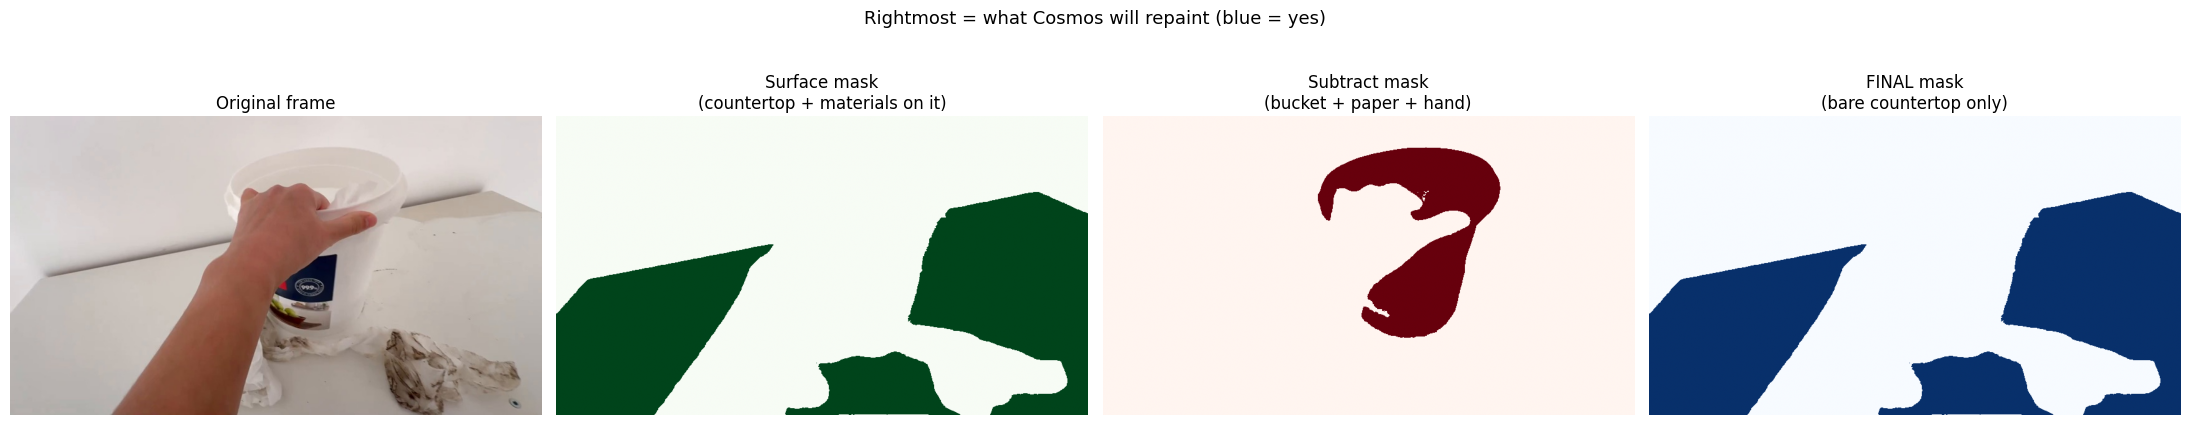
\includegraphics[width=\linewidth]{mask_strip.png}
\caption{Mask construction for the bucket clip. Left to right: original frame; SAM2 surface mask from the countertop box (includes objects on it); union of object masks from the bucket, paper and hand boxes; final mask $M$ after subtraction (Eq.~\ref{eq:mask}). Blue marks the pixels the renderer is meant to change.}
\label{fig:mask}
\end{figure}

\paragraph{Control maps}
Three further controls are derived from the source clip by the preprocessors shipped with Cosmos Transfer: a Canny edge video $c_{\mathrm{edge}}$~\cite{canny1986}, a monocular depth video $c_{\mathrm{depth}}$~\cite{depthanything}, and a heavily blurred RGB video $c_{\mathrm{vis}}$ that carries global color and lighting. The mask $M$ is supplied as the segmentation control $c_{\mathrm{seg}}$. It is a control signal, not a hard constraint: the model follows it to the degree set by the seg weight, and nothing in the pipeline forbids change outside $M$. Fig.~\ref{fig:controls} shows all four for one frame.

\begin{figure}[t]
\centering
\begin{subfigure}{0.24\linewidth}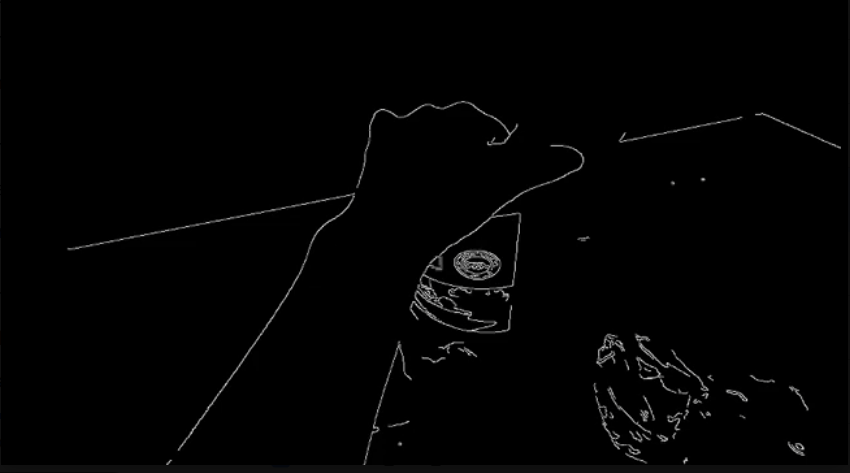
\includegraphics[width=\linewidth]{ctrl_edge.png}\caption{edge}\end{subfigure}\hfill
\begin{subfigure}{0.24\linewidth}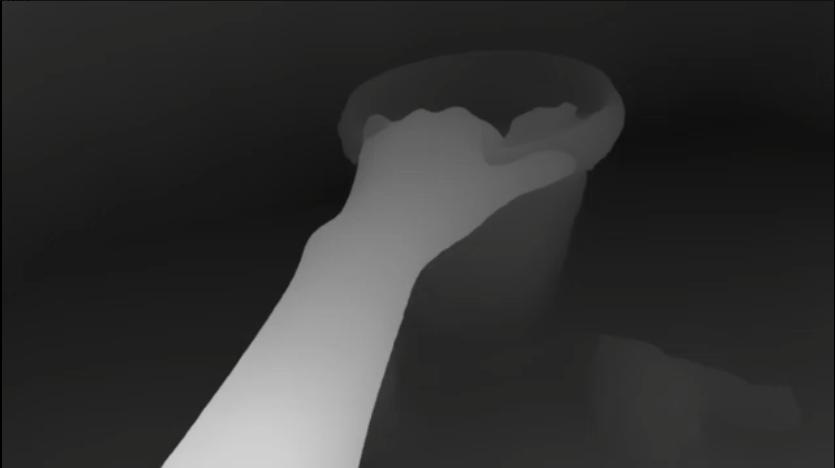
\includegraphics[width=\linewidth]{ctrl_depth.png}\caption{depth}\end{subfigure}\hfill
\begin{subfigure}{0.24\linewidth}
\includegraphics[width=\linewidth]{ctrl_vis.png}\caption{vis}\end{subfigure}\hfill
\begin{subfigure}{0.24\linewidth}
\includegraphics[width=\linewidth]{ctrl_seg.png}\caption{seg ($M$)}\end{subfigure}
\caption{The four control inputs to Cosmos Transfer~2.5 for one frame of the bucket clip. Edge fixes object outlines, depth fixes layout, vis fixes global color and lighting, and the segmentation control carries the subtraction mask.}
\label{fig:controls}
\end{figure}

\subsection{Generation}
\label{sec:generation}
Cosmos Transfer~2.5~\cite{cosmos25,cosmostransfer25} renders $V' = G(V, p, \{c_j\}, w)$ with 35 denoising steps and a guidance scale of 4. The control weights $w$ are the one set of hyperparameters we tuned, and Table~\ref{tab:weights} records the values and the failure that bounds each one. Edge and depth were fixed by failure modes on both sides; the only free choice was how to split the remaining budget between vis and seg. Vis stays near zero because any appreciable weight reasserts the source colors and undoes the recolor. Seg takes the rest. Seeds were not fixed, so a repeated render of the same inputs is not bitwise reproducible. Outputs are 60 frames at $854\times480$ and 4~fps, matching the input.

\begin{table}[t]
\centering
\caption{Control weights for Cosmos Transfer~2.5 and the failure that bounds each. Values are as passed to the model (they sum to 0.9; normalized to 1 they are 0.556, 0.222, 0.028, 0.194). Edge and depth were pinned by failures in both directions; vis and seg share what remains.}
\label{tab:weights}
\small
\begin{tabular}{@{}lS[table-format=1.3]ll@{}}
\toprule
Control & {Weight} & Lower bound failure & Upper bound failure \\
\midrule
edge  & 0.5   & objects lose shape & nothing changes \\
depth & 0.2   & layout drifts & scene flattens to a plane \\
vis   & 0.025 & (none observed) & recolor reverts \\
seg   & 0.175 & edits unlocalized & over-constrained \\
\bottomrule
\end{tabular}
\end{table}

\subsection{Routing action-level variations}
\label{sec:action}
The ontology's failure modes (``bucket tips over'') and state variations are not appearance edits; Transfer preserves the source motion by construction. For these we tried Cosmos Predict2 (2B, Video2World)~\cite{cosmospredict2}, which forecasts frames from a conditioning clip and a text description of what happens next. Sec.~\ref{sec:actionresults} reports the outcome.
